\documentclass[a4paper]{article}

%use the english line for english reports
%usepackage[english]{babel}
\usepackage[portuguese]{babel}
\usepackage[utf8x]{inputenc}
\usepackage{indentfirst}
\usepackage{graphicx}
\usepackage{verbatim}
\usepackage{color}
\definecolor{darkgray}{rgb}{0.41, 0.41, 0.41}
\definecolor{green}{rgb}{0.0, 0.5, 0.0}
\usepackage{listingsutf8}
\lstset{language=Prolog, 
	numbers=left,
	stepnumber=5,
	firstnumber=1,
	numberfirstline=true,
    basicstyle=\linespread{0.8}\ttfamily,
    keywordstyle=\color{blue}\ttfamily,
	showstringspaces=false,
    stringstyle=\color{red}\ttfamily,
    commentstyle=\color{green}\ttfamily,
	identifierstyle=\color{darkgray}\ttfamily,
    morecomment=[l][\color{magenta}]{\#},
	tabsize=4,
    breaklines=true,
    extendedchars=true,
	inputencoding=utf8x,
    escapeinside={\%*}{*)},
}
\lstset{literate=%
{│}{{$\mid$}}1
{↑}{{$\uparrow}$}1
{→}{{$\rightarrow}$}1
{↓}{{$\downarrow}$}1
{←}{{$\rightarrow}$}1
{─}{{-}}1
}
\usepackage[top=2cm, bottom=2cm, left=2cm, right=2cm]{geometry}

\begin{document}

%\setlength{\textwidth}{16cm}
%\setlength{\textheight}{22cm}

\title{\Huge\textbf{Dominup - Manual de Utilizador}}
\author{
Ângela Filipa Pereira Cardoso - up200204375 \\
Nuno Miguel Rainho Valente - up200204376 \\
}

\maketitle
%************************************************************************************************

Dominup é uma variação do jogo Dominó para 2 a 4 jogadores, em que, tal como o nome sugere, é possível colocar peças em cima de outras.

No típico Dominó existem 28 peças duplas numeradas de 0 a 6, à semelhança das faces de um dado. Já no Dominup há 36 peças duplas numeradas de 0 a 7, usando códigos binários: o ponto no centro representa 1, o circulo pequeno representa 2 e o circulo grande representa 4, como se pode ver na Figura~\ref{piece}. Este desenho das peças, juntamente com as regras do Dominup e de dois outros jogos, foram criadas por Néstor Romeral Andrés em 2014, sendo o conjunto publicado por nestorgames\footnote[1]{http://www.nestorgames.com}.

\begin{figure}[htbp]
\begin{center}

\includegraphics[scale=0.4]{piece.jpg}
\caption{Exemplo da peça $3 \cdot 6$.}
\label{piece}
\end{center}
\end{figure}

Existem dois tipos de colocação de peças no Dominup:
\begin{itemize}
	\item subir - a peça é colocada em cima de duas peças adjacentes que estejam ao mesmo nível, de forma a que os números da peça colocada sejam iguais aos que ficam por baixo (um em cada peça de suporte), tal como mostra a Figura~\ref{climb}.
	\item expandir - a peça é colocada na superfície de jogo, de forma a que fique adjacente e ortogonal a pelo menos uma peça já colocada, como, por exemplo, as duas peças já colocadas na Figura~\ref{climb}.
\end{itemize}

\begin{figure}[htbp]
\begin{center}
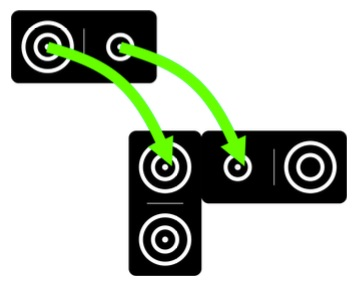
\includegraphics[scale=0.3]{climb.jpg}
\caption{Exemplo de um posicionamento a subir válido.}
\label{climb}
\end{center}
\end{figure}

Tal como no Dominó, as regras são relativamente simples. Começa-se por distribuir as peças aleatoriamente e de forma equilibrada pelos jogadores, mantendo a face voltada para baixo. 

O jogador com o duplo 7 inicia o jogo, colocando essa peça no centro da superfície de jogo e determinando a ordem dos restantes jogadores, que é dada pelo sentido contrário ao ponteiro dos relógios. 

Começando no segundo, cada jogador, na sua vez, realiza ambos os passos seguintes:
\begin{enumerate}
	\item Enquanto for possível, coloca peças a subir, podendo escolher a ordem em que o faz;
	\item Se ainda tiver alguma peça, coloca-a a expandir.
\end{enumerate}

Se, no final da sua vez, o jogador ficar sem peças, é declarado vencedor e o jogo termina. Alternativamente, os restantes jogadores podem continuar, de forma a determinar o segundo, terceiro e quarto lugares.

Na Figura~\ref{example} pode ser observado um possível jogo de Dominup a decorrer.

\begin{figure}[htbp]
\begin{center}
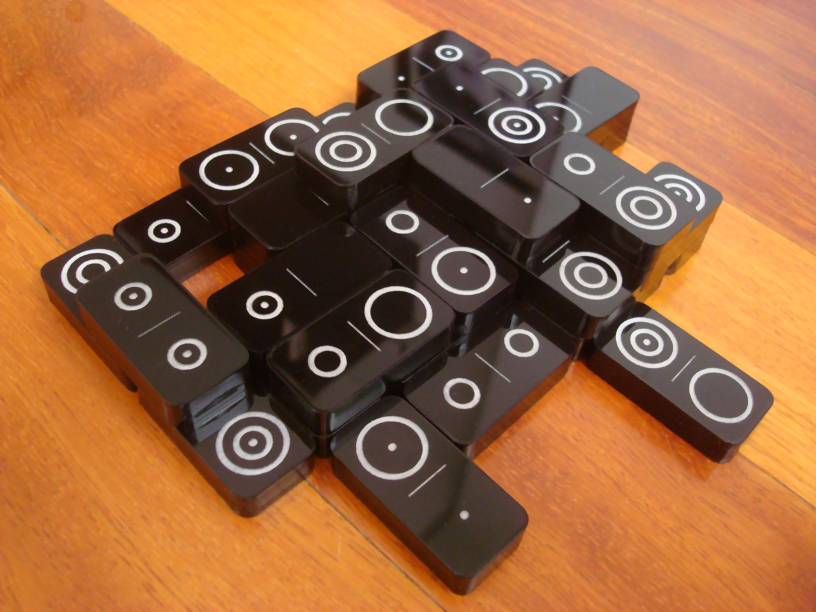
\includegraphics[scale=0.2]{example.jpg}
\caption{Exemplo de um jogo de Dominup.}
\label{example}
\end{center}
\end{figure}

Na nossa implementação gráfica do jogo, é possível escolher, utilizando menus, se pretendemos um novo jogo ou continuar um jogo previamente salvado. Em caso de novo jogo, este pode ser humano vs humano, humano vs computador ou computador vs computador. Para cada jogador humano deve ser fornecido um nome e para cada jogador computador, deve ser escolhido um nível de dificuldade entre fácil e difícil. A Figura~\ref{menu} tem um exemplo do menu inicial de jogo.

\begin{figure}[htbp]
\begin{center}
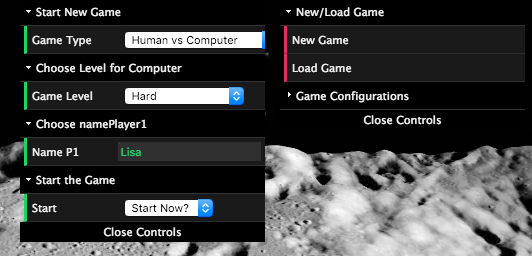
\includegraphics[scale=0.4]{menu.png}
\caption{Menu inicial.}
\label{menu}
\end{center}
\end{figure}

Uma vez iniciado o jogo, as jogadas do computador são automáticas. Os jogadores humanos devem selecionar uma das suas peças, clicando sobre ela e depois selecionar duas posições do tabuleiro. A primeira posição selecionada será para o lado esquerdo da peça e a segunda para o lado direito. Um exemplo com o interface de jogo pode ser observado na Figura~\ref{interface}.

\begin{figure}[htbp]
\begin{center}
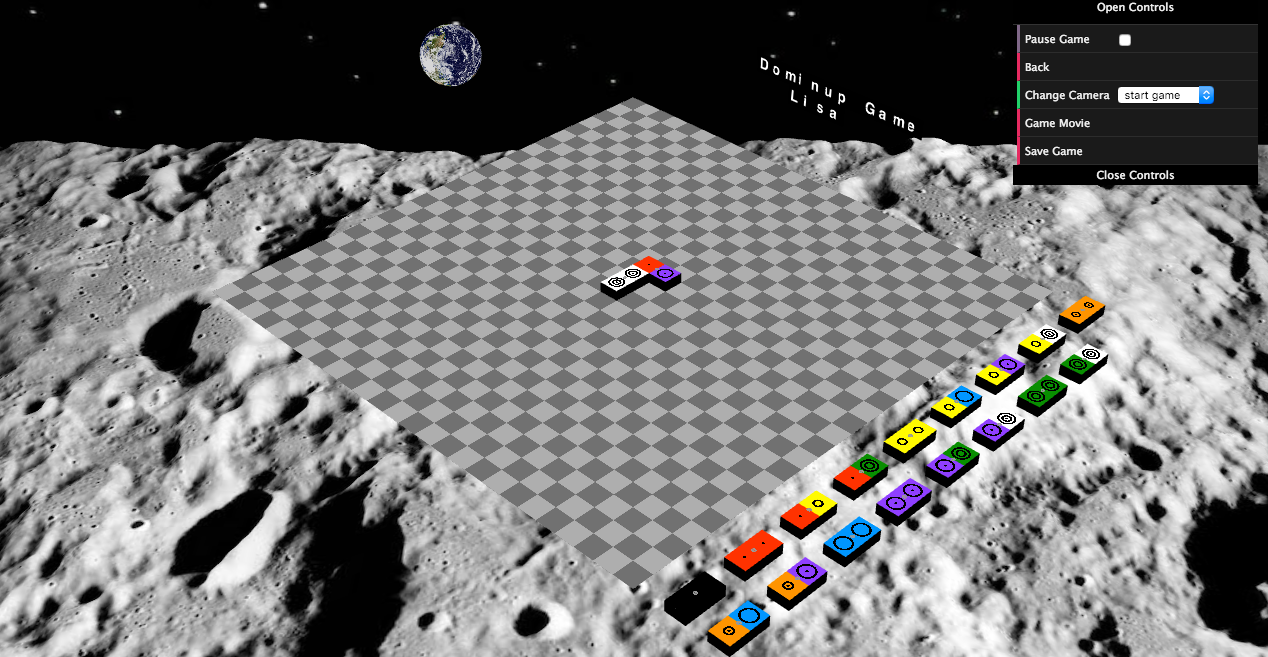
\includegraphics[scale=0.3]{game.png}
\caption{Interface de jogo.}
\label{interface}
\end{center}
\end{figure}

\end{document}
